\appendix

\section{Structural Comparison}
\label{app:structural}

\begin{table}[h]
\centering
\small
\begin{tabular}{p{2.2cm}p{2.3cm}p{2.3cm}}
\toprule
\textbf{Dimension} & \textbf{Tool-Use} \cite{paladin2025} & \textbf{Embodied} \\
\midrule
Error signal & Discrete (API error codes) & Diffuse (wrong object, wrong room) \\
Observability & Explicit (stack trace) & Silent (no error msg) \\
Recovery scope & Local (retry call) & Global (replan) \\
Feedback & Immediate & Delayed \\
Error locality & Single step & Cascading \\
\bottomrule
\end{tabular}
\caption{Structural comparison: tool-use vs.\ embodied planning. Error injection benefits from discrete, observable, locally recoverable errors.}
\label{tab:structural}
\end{table}

\section{Training Dynamics}
\label{app:training_dynamics}

Figure~\ref{fig:training_curves} shows training loss curves across conditions. At $\geq$25\% injection, models achieve lower final training loss than Vanilla (TaxEI-50\%: 0.259 vs.\ Vanilla: 0.288) despite worse evaluation performance (\S\ref{sec:paradox}). At 10\% injection, training loss (0.308) remains above Vanilla.

\begin{figure}[t]
\centering
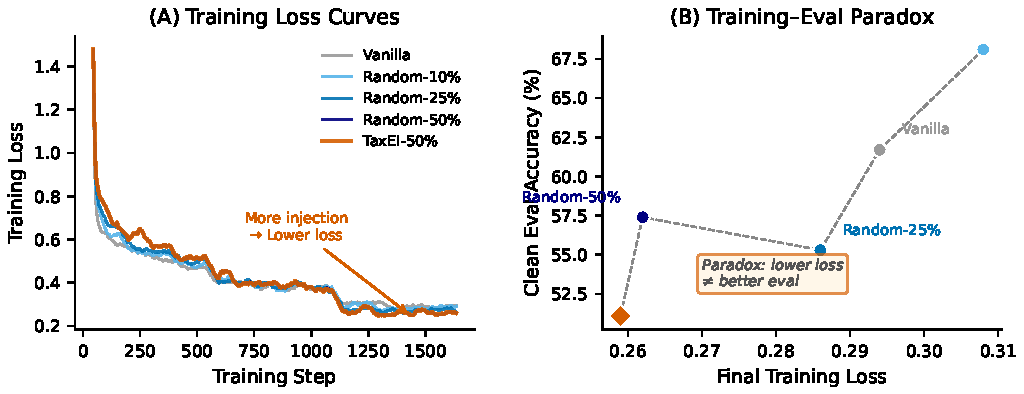
\includegraphics[width=\columnwidth]{figures/paper/fig_app_training_curves.pdf}
\caption{Left: training loss curves. Right: final loss vs.\ eval accuracy---lower loss corresponds to worse performance at $\geq$25\% injection.}
\label{fig:training_curves}
\end{figure}

\section{Per-Task Cross-Analysis}
\label{app:cross_analysis}

For seed=42, the $\sim$6.4pp aggregate gap between TaxEI and Random at each dose point corresponds to $\approx$3 tasks on a 47-task evaluation. This consistency does not hold across seeds: at 25\% the 3-seed mean gap is 8.5pp, at 50\% it is 2.1pp. Cross-dose analysis reveals this is a discretization coincidence: zero tasks appear as TaxEI-penalty in all three dose points (10\%, 25\%, 50\%). The specific tasks that flip between conditions rotate across doses---9 different tasks contribute to the penalty, with no single task appearing at all three levels.

\section{Version Discrepancy}
\label{app:version}

Our evaluation pipeline evolved from v3 to v4 during development. The v3 vanilla baseline (74.5\%, seed=42) was higher due to a format mismatch. The v3$\to$v4 transition involved three changes: (1)~prompt format alignment from ChatML to tool-format, (2)~sample count increase from 4{,}176 to 4{,}358 due to improved trajectory collection, and (3)~seed handling standardization. The 12.8pp drop (74.5\%$\to$61.7\%) is attributable primarily to the format alignment. All three conditions (Vanilla, TaxEI, Random) were trained and evaluated under the same v4 pipeline, ensuring fair internal comparisons.
